\subsection{Taxi Speed}
We first investigate the average speed $\overline{speed}$ in each status. If taxi $i$ drives in occupied status for a distance $d$ using time $t$, then its average speed in this status is $d/t$.
From March 3 to 7, 2011, ${\overline{speed}_{vacant}} = 3.627 m/s$, while ${\overline{speed}_{occupied}}=7.083 m/s$. Clearly, occupied taxis drive faster. To further investigate the cumulative speed distribution, proportion for every $\overline{speed}$ section is calculated and plotted in Fig.~\ref{figure_speed_distribution}. Here, a point at $(5,0.2)$ means $20\%$ records fall in the range $[0,5)km/h$. We also fit the speed to model the microscope behavior (will be discussed in Section \ref{section_modeling}). Fig.~\ref{figure_speed_distribution} shows that $\overline{speed}$ distribution differs for each status and with strong regularity for each status.

\begin{figure}[!h]
\centering
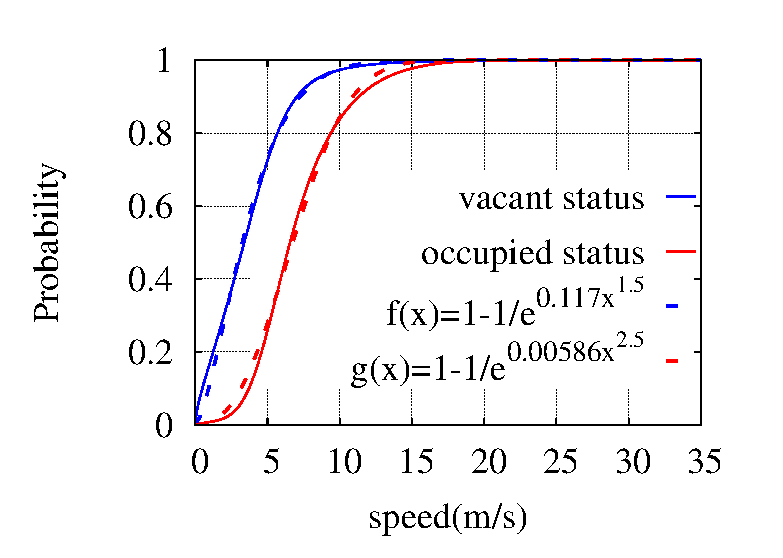
\includegraphics[width=0.4\textwidth]{figures/fit/speedfit.eps}
\caption{Speed distributions for vacant and occupied statuses.}\label{figure_speed_distribution}
\end{figure}




